%----------------------------------------------------------------------------
\chapter{Háttérismeretek}\section{A monitorozás alapjai}

Egy monitor feladata az, hogy futási időben egy rendszert megfigyeljen, elemezzen és adott követelmények alapján felismerje a rendszer helytelen viselkedését.
Ezt a helytelen viselkedést jelzi a rendszernek, de néhány esetben a rendszer működését is befolyásolhatja.
Ez egy kritikus rendszernél különösen fontos lehet hiszen, egy ilyen rendszernél elvárt, hogy folyamatosan biztonságosan tudjon működni.
Ezen kívül, a monitornak időmérésre is szüksége van, mert a követelmény tartalmazhat időzítéseket is.
Az \ref{introductory_figure} ábra bemutatja a monitorozás koncepcióját.

\begin{figure}[!ht]
    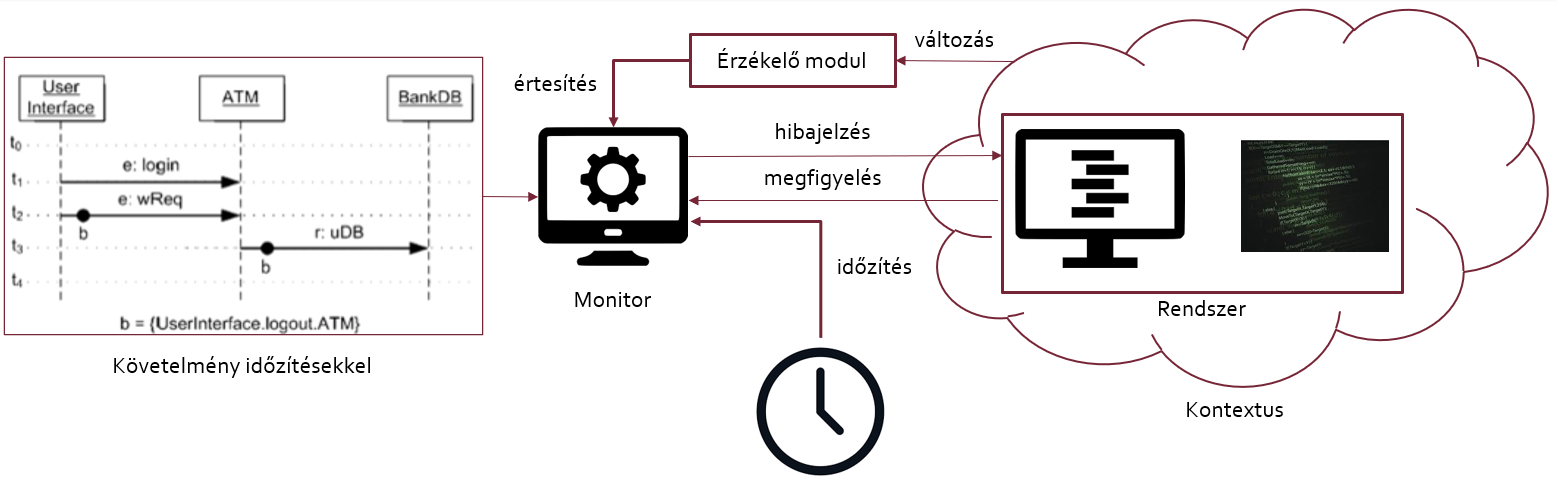
\includegraphics[width=150mm, keepaspectratio]{figures/introductory_figure.png}
    \caption{Kontextusfüggő rendszerek monitorozása időzítési feltételekkel.}
    \label{introductory_figure}
\end{figure}

Több monitorozási módszert ismerünk.
Ilyen például az „\textit{online}” [11] monitorozás.
Ebben az esetben a rendszernek olyan érzékelői vannak, amelyek képesek a rendszer viselkedését detektálni, és továbbítani azt egy feldolgozó egységnek.
Ez utóbbi, a kapott adatok alapján, el tudja dönteni, hogy a rendszer helyesen működik-e, illetve amennyiben hibát érzékel, azt képes jelezni.
Az olyan monitort, amely a hiba érzékelését követően megpróbálja a hibát helyreállítani, „beavatkozó” monitornak hívjuk.
A „nem beavatkozó” monitor pedig csak a hibát képes jelezni.

A fentiekben leírt monitorozási módszernek a párja az „\textit{offline}” [11] monitorozás.
Ennél a módszernél a regisztrált viselkedés elemzése nem futásidőben, hanem azon kívül (futás után) történik.

A szcenárió alapú monitorozás során a kommunikáció megfigyelésével szeretnénk felismerni a problémákat a rendszerünkben.
A rendszerben lévő objektumok közti interakciókat, üzeneteket fogja megfigyelni a monitor.
A követelményt szcenárió formájában adjuk meg az üzenet szekvenciák specifikálásával.
Szekvencia diagramok segítségével egyszerűen megadhatunk ilyeneket.
A diagramokat a későbbiekben olyan alakra kell majd hoznunk, hogy abból a monitor létrehozható legyen.

\section{Időfüggő viselkedés specifikálására alkalmas formalizmusok áttekintése [1] [2] [5] [6] [8]}
\subsection{MSC - Message Sequence Chart [6] és UML - Unified Modelling Language [8]}

Az egyik legelterjedtebb szcenárió alapú modellezésre használt vizuális formalizmus a \textit{Message Sequence Charts (MSC)}.
A nyelv célja két, vagy több üzeneteket cserélő objektum között az interakciónak a leírása.
A \textit{Unified Modelling Language (UML)} 2.0 szekvencia diagram leíró részét nagyban inspirálta ez a nyelv.
Az \textit{MSC} főbb elemei:

\begin{itemize}
\item \textit{MSC head}, \textit{lifeline} és \textit{end}
\item Objektum létrehozása
\item Üzenet csere
\item Függvényhívás és válasz
\item \textit{Timer}-ek
\item Idő intervallumok
\item Összetett szerkezetek: \textit{alt}, \textit{opt}, \textit{parallel}, \textit{loop} (\textit{high-MSC})
\end{itemize}

Az összetett szerkezetek a \textit{high-MSC (h-MSC)} nevű \textit{MSC} kiterjesztésben találhatók.

Ezzel a nyelvvel már könnyedén lehet a szcenárióban lévő üzeneteket specifikálni, és azokat a rendszer komponenseket, amelyek ezeket az üzeneteket egymásnak küldik.

Az \textit{UML} és az \textit{MSC} sokban hasonlítanak, de az alapelveik különbözőek.

\textit{MSC}-ben a függőleges vonalak („\textit{lifeline}”-ok) autonóm entitásokat képviselnek, míg a szekvencia diagramok esetén ezek egy-egy objektumot reprezentálnak.
\textit{MSC} esetén az entitásoknak nem szükséges ugyanazon a számítógépen lenniük.

\textit{MSC}-ben egy átmenet egy aszinkron üzenetet reprezentál, amely két entitás között jött létre, míg az \textit{UML} szekvencia diagram leíró nyelvében, egy átmenet egy függvényhívást jelent.

Az \textit{MSC}-nek sajnos sok hiányossága is tapasztalható.
Hiányzik belőle az üzenetek típusossága.
Egy követelmény megfogalmazásakor fontos, hogy meg tudjuk mondani, melyek az elvárt üzenetek vagy, hogy melyek jelentenek hibát.
Az is nagy hiányosságnak számít, hogy az üzenetekre nem lehetséges megkötéseket megadni.
Ez megnehezíti egy követelmény leírását is.

\begin{figure}[!ht]
    \centering
    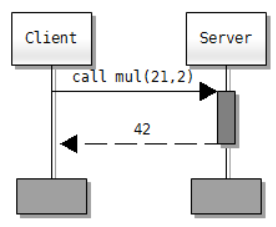
\includegraphics[width=80mm, keepaspectratio]{figures/msc_example.png}
    \caption{Példa MSC diagram.}
    \label{msc_example}
\end{figure}

A \ref{msc_example} ábrán megtekinthető egy példa MSC diagram.

\clearpage\subsection{MTL - Metric Temporal Logic}

A temporális logikák olyan formális rendszerek amelyekkel kijelentések igazságának logikai időbeli változását vizsgálhatjuk.
A kijelentések időbeli vizsgálásához temporális operátorokat használunk: \textit{mindig}, \textit{valamikor}, \textit{mielőtt}, \textit{addig, amíg}, \textit{azelőtt, hogy}, \textit{stb...}

A temporális logikákat két osztályba sorolhatjuk:
\begin{itemize}
    \item \textit{lineáris}
    \item \textit{elágazó}
\end{itemize}
A lineáris temporális logikáknál a modell egy lefutását vizsgáljuk.
A logikai idő egy állapotsorozatnak tekintjük, ahol minden állapotnak egy rákövetkezője van.
Az elágazó temporális logikáknál viszont az összes lehetséges végrehajtást tekintjük.
A lineárissal ellentétben itt egy állapotnak több rákövetkezője is lehet és a logikai idő egy fa alakjában jelenik meg.

Az \textit{MTL} egy lineáris temporális logika, amellyel logikai jelek időzítésbeli tulajdonságait specifikálhatjuk.
Logikai jelek tulajdonságait specifikálhatjuk vele az időben.

A szintaxisa a \textit{Linear Temporal Logic}-hoz hasonlít:
\begin{itemize}
    \item atomi kijelentések véges halmaza \textit{AP}
    \item $\neg$ és $\lor$ logikai operátorokat
    \item $U_I$ (\textit{Until}) temporális modális operátor, ahol \textit{I} egy nem negatív számokból álló intervallum
    \item $S_I$ (\textit{Since}) temporális modális operátor
\end{itemize}

A $p U_I q$ („\textit{p Until q}”) kifejezés akkor lesz igaz $t$ időben, ha létezik olyan $t' \in I + t$ idő amire a következők teljesülnek:
\begin{itemize}
    \item $t'$ időben $q$ igaz
    \item minden egyes $t'' \in T$ ahol $t < t'' < t'$ és $T 	\subseteq {R} _{+}$ időben $p$ igaz
\end{itemize}

A $p S_I q$ („\textit{p Since q}”) kifejezés akkor lesz igaz $t$ időben, ha létezik olyan $t' \in I - t$ idő amire a következők teljesülnek:
\begin{itemize}
    \item $t'$ időben $q$ igaz
    \item minden egyes $t'' \in T$ ahol $t' < t'' < t$ időben $p$ igaz
\end{itemize}

Például a $p U_{1} q$ \textit{MTL} formula azt követeli meg, hogy minden egy időegységgel előtti állapotban ahol $q$ teljesül, $p$-nek teljesülnie.

A \textit{past-MTL} megfelel a teljes \textit{MTL}-nek az \textit{Until} operátor kivételével.
Hasonlóan, a \textit{future-MTL} a teljes \textit{MTL} a \textit{Since} operátor nélkül.

Az egyes cikkekben változó, hogy az \textit{MTL}-t hogyan definiálják.
Az \textit{MTL} megegyezik az előbbi \textit{future-MTL}-el vagy a teljes szintaxissal van definiálva.

\subsection{MITL - Metric Interval Temporal Logic}

Az \textit{MITL} egy részhalmaza az \textit{MTL}-nek.
Az \textit{MITL} temporális logika nem képes a következő követelmény megadására: „\textit{A} esemény pontosan öt időegység óta történt”.
Ezt gond nélkül megfogalmazhatjuk \textit{MTL}-ben.
\textit{MITL}-ben csak a következőt tudjuk leírni: „\textit{A} esemény négy és öt időegység között történt”.

Például a $p U_{0,1} q$ \textit{MITL} formula azt fejezi ki, hogy minden állapotot amiben $q$ teljesül és egy időegységnyi távolságra van előtt, $p$-nek kell teljesülnie.

A temporális logikák nagy hátránya az, hogy ha hosszú szekvenciális követelményeket szeretnénk leírni akkor nagyon hosszú és bonyolult formulákat kell használnunk.
Ezeket viszont nagyon nehéz megírni és nehezen olvasható ki belőlük a követelmény.
A szcenárió alapú formalizmusok sokkal intuitívabbak és ilyen követelmények megadására sokkal alkalmasabbak.
Egy szcenárió egy konkrét lefutást ír le, amíg a temporális logikák egy állapotára tud követelményt specifikálni.

\subsection{PSC – Property Sequence Chart}
%----------------------------------------------------------------------------
A \textit{Message Sequence Chart}-nak nagyon sok hiányossága van.
Nem lehet vele megkötéseket definiálni vagy egy üzenetről eldönteni, hogy az egy elvárt vagy nem kívánt üzenet.
Ebből kifolyólag az \textit{MSC} nem egy alkalmas nyelv arra, hogy az üzenet szekvenciáinkat részletesebben specifikálni tudjuk vele.

\begin{table}[ht]
    \centering % used for centering table
    \begin{tabular}{ |c|c|c| } % centered columns (4 columns)
    \hline
    \textbf{Tulajdonság} & \textbf{MSC} & \textbf{PSC} \\ [0.5ex] % inserts table
    %heading
    \hline % inserts single horizontal line
    \hline
    Nem kivánt üzenet & - & \textit{Fail message} \\ % inserting body of the table
    \hline
    Elvárt üzenet & - & \textit{Required message} \\
    \hline
    Sima üzenet & \textit{Default message} & \textit{Regular message} \\
    \hline
    Megkötött sorrendezés & - & \textit{Strict sequencing} \\
    \hline
    Gyenge sorrendezés & \textit{Seq} & \textit{Loose sequencing} \\
    \hline
    Üzenet megkötések & - & \textit{Constraint} \\
    \hline
    Alternatív lehetőségek & \textit{h-MSC} & \textit{Alternative operator} \\
    \hline
    Párhuzamos művelet & \textit{h-MSC} & \textit{Parallel operator} \\
    \hline
    Ciklus & \textit{h-MSC} & \textit{Loop operator} \\
    \hline %inserts single line
    \end{tabular}
    \label{psc_táblázat} % is used to refer this table in the text
    \caption{Az \textit{MSC} összehasonlítása a \textit{PSC}-vel} % title of Table
\end{table}

A \textit{Property Sequence Chart}[1] az \textit{MSC} egy kiterjesztése.
Sok új elemet vezet be ami nincs az \textit{MSC}-ben, melyek megtekinthetők a \ref{psc_táblázat} táblázatban, mint az üzenet típusokat: sima üzenet (e), elvárt üzenet (r) és nem kívánt üzenet (f).
Így specifikálhatjuk, hogy mely üzenetek azok amik helyes viselkedésre utalnak és azok amelyek nem.
Szigorú sorrendezésre is ad megoldást a \textit{PSC}, ami azt jelenti, hogy megadhatjuk explicit az üzenetek sorrendjét a követelményünkben.
A gyenge sorrendezés és a szigorú sorrendezés között az a különbség, hogy szigorú sorrendezés a szekvenciában lévő üzenetek között nem jelenhet meg más üzenet.
Gyenge sorrendezésnél megengedjük, hogy az üzenetek között más üzenetek is megjelenjenek, amelyeket nem vettünk be a követelménybe.
A \textit{PSC}-ben egy üzenetre megkötést is rakhatunk.
Megadhatjuk, hogy melyek azok az üzenetek amik nem kívántak az üzenetünk észlelése előtt vagy után.
A különböző \textit{PSC} tulajdonságok megtalálhatok a \ref{psc_elemek} ábrán.

A nyelv a következő tulajdonságokat támogatja:
\begin{itemize}
    \item \textit{Sima üzenet (e)}: egy üzenet a szcenárióban, amely ha nem történik meg az a monitor szempontjából nem jelent hibát.
    Viszont ha megjelenik, akkor a szcenárióban utána következő üzenetek ellenőrzésére kell áttérni.
    Egy előfeltételt reprezentál.
    \item \textit{Elvárt üzenet (r)}: egy üzenet amelynek elmaradása hibajelzéshez kell vezessen.
    \item \textit{Nem kívánt üzenet (f)}: amennyiben a monitor egy ilyen üzenetet detektál, akkor hibát jelez.
    \item \textit{Üzenet megkötés (constraint)}: Egy üzenetre lehet megkötést is helyezni.
    Egy megkötés több üzenetet tartalmazhat.
    Két fajta megkötést definiál a nyelv: múlt- és jövőbéli.
    A múltbéli üzenet megkötés esetén, az üzenetünk megtörténte előtt, a megkötésben szereplő üzenetek egyike se történhet meg.
    Jövőbéli megkötés esetén, pedig az üzenetünk megtörténte után nem történhetnek meg a megkötésben szereplő üzenetek.
    \item \textit{Megkötött sorrendezés (strict ordering)}: A \textit{PSC} az üzenet lefutási sorrendjének a specifikálására is lehetőséget ad.
    Egy „a” üzenet megtörténte után, egy adott „b” üzenetnek kell bekövetkeznie.
    Ha „b” üzenet helyet egy másik üzenet követi az „a” üzenetet, akkor a monitor hibát jelez.
    Nem megkötött sorrendezés esetén nem jelent hibát ha „a” és „b” üzenet között más üzenetek is megjelennek.
\end{itemize}

A nyelv támogat összetett szerkezeteket is:

\begin{itemize}
    \item \textit{Alt operátor}: az \textit{alt} operátorral alternatív üzenet szekvenciákat lehet definiálni.
    \item \textit{Par operátor}: a \textit{par} operátorral megadható üzenet szekvenciák párhuzamos futása.
    \item \textit{Loop operátor}: a \textit{loop} operátorral megadhatjuk, hogy egy üzenet szekvencia többször is lefuthat egymás után.
\end{itemize}

Egy üzeneten egyszerre megkötés és sorrendezés is lehet.
Az üzenetek típusát a címkéjén lévő karakterrel jelöljük.
Az „e” karakter jelzi, hogy az üzenet sima, az „r” karakter az elvárt üzenetet jelenti, az „f” pedig a nem kívánt üzenetet.
Azt meg kell jegyezni, hogy nem kívánt üzenetekre nem lehet jövőbéli megkötéseket rakni.
Ezen kívül, ha egy üzeneten megkötött sorrendezést alkalmazunk, akkor nem lehet rajta múltbéli megkötés.

A megkötéseket egy ponttal jelöljük, amit az átmeneten helyezünk el.
Ha a pont az átmenet elején van (a feladóhoz közel), akkor az múltbéli megkötést jelöl.
Ha pedig a végén helyezkedik el, akkor a jövőbéli megkötést jelöli.
A megkötésben lévő üzeneteket egy lista formájába lehet megadni ’{’ ’}’ jelek közt, a következő módon: <megkötés neve> = {C1.I1.Cj, ..., Ck.In.Ct}, ahol az üzenetek vesszővel elválasztva, „\textit{Feladó.Üzenet.Címzett}” formában szerepelnek.
A specifikált megkötés nevét pedig az átmeneten lévő pont alá írjuk.

Az üzenetek megkötött sorrendezésének jelölésénél az objektum „\textit{lifeline}” vonalát az érintett átmenetek közt folytonossá változtatjuk

\begin{figure}[!ht]
    \centering
    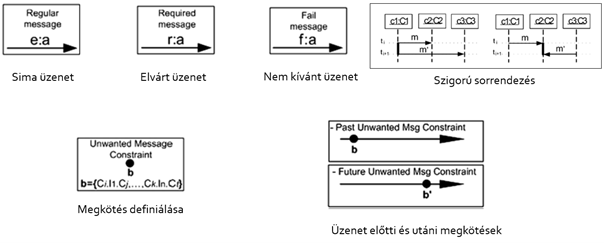
\includegraphics[width=150mm, keepaspectratio]{figures/2abra.png}
    \caption{A \textit{PSC} különböző elemei [1].}
    \label{psc_elemek}
\end{figure}

Az üzeneteket a következő formában adjuk meg: \textit{Feladó.Üzenet.Címzett}.

\begin{figure}[!ht]
    \centering
    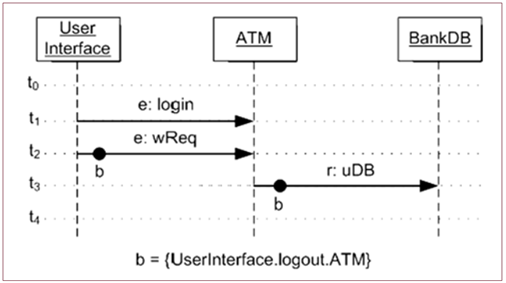
\includegraphics[width=130mm, keepaspectratio]{figures/3abra.png}
    \caption{\textit{PSC} diagram egy \textit{ATM} rendszer működésének ellenőrzésére[1].}
    \label{psc_példa}
\end{figure}
A \ref{psc_példa} ábrán láthatunk egy példát arra, hogy egy követelményt hogyan lehet definiálni.
Ez a \textit{PSC} diagram egy \textit{ATM} rendszer működését specifikálja.
Először a felhasználó egy \textit{login} üzenettel bejelentkezik az \textit{ATM}-be majd egy \textit{wReq} üzenettel egy lekérdezést hajt végre.
Ezen az üzeneten van egy megkötés, az üzenet előtt nem történthet kijelentkezés, \textit{logout}.
Az \textit{ATM} ezután, ha nem történt \textit{logout} egy elvárt üzenetet küld a \textit{Bank} adatbázisába.

A szcenárióink specifikálására így rendelkezésünkre áll egy grafikus nyelv.
A következőkben az lesz a feladatunk, hogy ezekből a diagramokból valósítsuk meg a monitor kódjának generálását.

%----------------------------------------------------------------------------
\section{A TPSC bemutatása}
%----------------------------------------------------------------------------
A \textit{TPSC}[2] a \textit{PSC}-nek egy kiterjesztése.
A \textit{PSC} üzenetekre időzítési feltételeket specifikálhatunk.

\begin{figure}[!ht]
    \centering
    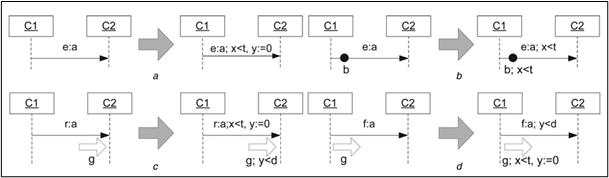
\includegraphics[width=150mm, keepaspectratio]{figures/4abra.png}
    \caption{\textit{PSC} kiterjesztése időzítési feltételekkel[2].}
    \label{psc_clock_improvement}
\end{figure}

A \textit{TPSC} óraváltozókat (pl. x, y) használ az időzítéshez.
Ezekre meg lehet adni feltételeket, valamint az óraváltozót lehet nullázni.
A nullázással adott eseménytől (pl. üzenet vételétől) kezdve indul az időzítés, majd rákövetkező események időbeliségét ez alapján lehet ellenőrizni.

A \ref{psc_clock_improvement} ábrán látható, hogy például az \textit{e: a} sima üzenet \textit{e: a; x < t, y := 0} üzenetre bővül.
Elvárjuk, hogy az \textit{a} üzenet \textit{t} idő előtt történjen meg és egy \textit{y} óraváltozót nullázunk.
Az \textit{e: a} üzenet egy sima üzenet, szóval ha nem történik meg a specifikált idő intervallumban az nem jelent hibát.
Viszont \textit{r: a} üzenetnél ugyanilyen feltétel mellett már elvárt, hogy \textit{t} időn belül megtörténjen. \textit{f: a} üzenet esetében viszont akkor jelez hibát a monitor, ha üzenet megtörtént \textit{t} időn belül.

Egy múltbeli vagy jövőbeli megkötésre is meg lehet adni időzítési feltételt.
Így megadhatjuk, hogy mennyi ideig nem szabad jönnie a megkötésben szereplő nem kivánt üzenetek egyikének.
Ha a feltételben megadott idő után történik akkor az nem jelent hibát a monitor szempontjából.

% !TeX spellcheck = hu_HU
% !TeX encoding = UTF-8
% !TeX program = xelatex
%----------------------------------------------------------------------------
\clearpage\section{TPSC szcenárió alapú automata konstrukció}
%----------------------------------------------------------------------------

A monitorozás alapja, hogy \textit{TPSC} szcenáriókból időzített automatákat (\textit{Timed Automata}) tudjunk készíteni.
Egy \textit{TA} állapotokból, elfogadó állapotokból, feltételekből, akciókból és bemenetekkel címkézett állapotátmenetekből áll.
Ezek a következő sorrendbe jelennek meg az állapotátmeneteken: bemenet, feltétel és akció.
A bemenet lehet egy konkrét esemény, ilyen például az „\textit{a}” üzenet, vagy több eseményre utaló kifejezés.
Például a „\textit{!a}” kifejezés minden olyan üzenet amelyik nem az „\textit{a}” üzenet.
Egy feltétel a mi esetünkben egy időzítési feltétel, ezekhez óraváltozókat használunk.
Egy akció lehet például egy ilyen óraváltozónak a nullázása.
Ha a feltétel teljesül és az adott üzenet illeszkedik az állapotátmeneten lévő bemenetre, akkor az megvalósulhat és a rajta lévő akció megtörténik.
Az automata akkor fogad el egy bemenet sorozatot, ha ennek során elérünk az automata végállapotába.
Ha hibaállapotot érünk el, akkor az a monitor szempontjából hibát jelent.
Az alapelv az, hogy minden \textit{TPSC} elemhez tartozik egy minta automata (\textit{pattern}) ami leírja a szemantikáját.
Például a \ref{tpsc_sima} és \ref{tpsc_elvárt} ábrákon láthatóak a különböző \textit{PSC} üzenetekhez tartozó minták.

\begin{figure}[!ht]
    \centering
    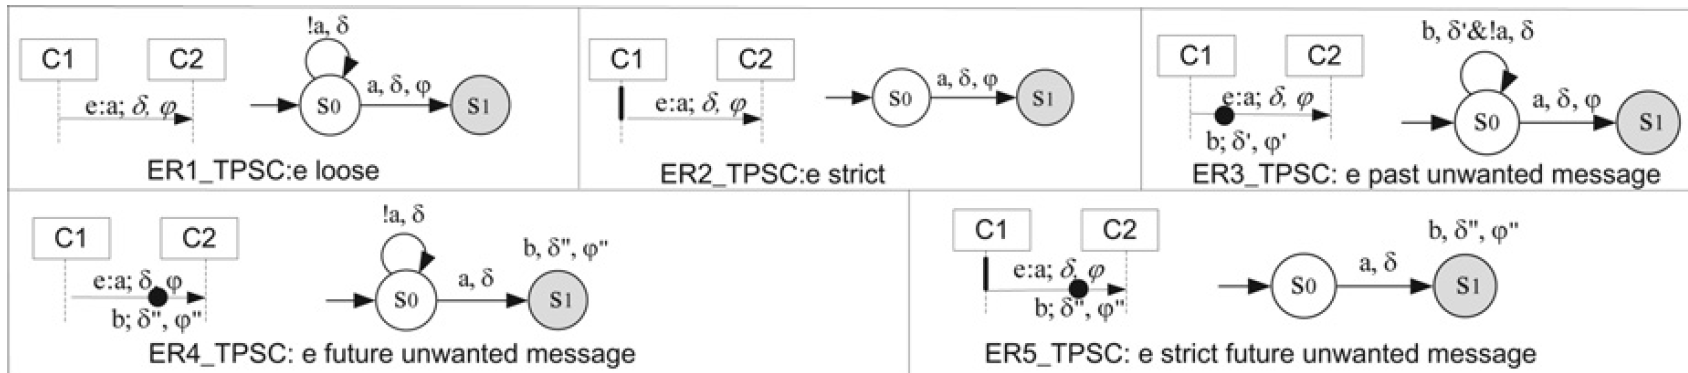
\includegraphics[width=150mm, keepaspectratio]{figures/sima_tpsc.png}
    \caption{Sima üzenetekhez tartozó minták [2].}
    \label{tpsc_sima}
\end{figure}

\begin{figure}[!ht]
    \centering
    \includegraphics[width=150mm, keepaspectratio]{figures/elvárt_tpsc.png}
    \caption{Elvárt üzenetekhez tartozó minták [2].}
    \label{tpsc_elvárt}
\end{figure}

\begin{figure}[!ht]
    \centering
    \includegraphics[width=150mm, keepaspectratio]{figures/példa_tpsc.png}
    \caption{Elvárt múltbéli megkötést tartalmazó üzenethez tartozó minta [2].}
    \label{tpsc_példa}
\end{figure}

A minta automatánkban található szürke állapotok reprezentálják a végállapotokat.
A megkötéseket a nem kívánt üzenetek negáltjainak az \textit{ÉS} kapcsolata.
Az időzített automatán egy átmenet formájában jelennek meg.
Például az \ref{tpsc_példa} ábrán lévő automata mintán látható „b, $\delta ’\&!a, \delta$” címkéjű hurokélen, a „b” címke minden olyan üzenetnek felel meg, amelyek nincsenek a megkötésben lévő nem kivánt üzenetek halmazában.
A címke teljes jelentése az, hogy ha $\delta$’ időn belül nem jött nem kivánt üzenet és $\delta$ időn belül nem az „a” üzenet jött akkor maradjunk az \textit{s0} állapotban.
A „a, $\delta$” címkéjű átmenet az „s0” állapotból az „s1” végállapotba mutat.
Az átmenet akkor valósul meg ha „a” üzenet érkezik és „$\delta$” időzítési feltétel igaz.
Ebben az esetben teljesül a feltétel.
Ha viszont a megkötésben szereplő nem kívánt üzenet érkezik és „$\delta$’” igaz vagy „a” üzenet érkezik „$\delta$” előtt vagy bármilyen üzenet érkezik „$\delta$” után, akkor a hibaállapotba lépünk át.

Ezekből az automata részekből lesznek meghatározott illesztési szabályokkal a szcenárióhoz tartozó teljes időzített automaták.
Ennek az az alapelve, hogy a szcenárión végig menve az előző minta végállapotát a következő minta kezdőállapotával kell egyesíteni.
Ezt a folyamatot mutatják be a \ref{tpsc_subset}, \ref{tpsc_used_patterns} és \ref{created_automaton} ábrák.
Ebben a példában a \ref{tpsc_used_patterns} ábrán lévő baloldali automata „s1” állapotát kellett egyesíteni a jobb oldali automata „s0” állapotával.

\begin{figure}[!ht]
    \centering
    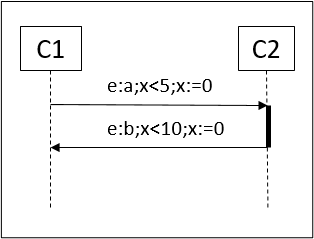
\includegraphics[width=60mm, keepaspectratio]{figures/7abra.png}
    \caption{TPSC részlet.}
    \label{tpsc_subset}
\end{figure}

\begin{figure}[!ht]
    \centering
    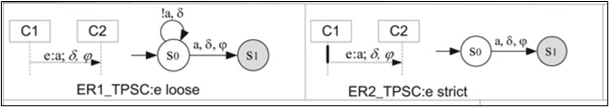
\includegraphics[width=150mm, keepaspectratio]{figures/8abra.png}
    \caption{Alkalmazott automata minták.}
    \label{tpsc_used_patterns}
\end{figure}

\begin{figure}[!ht]
    \centering
    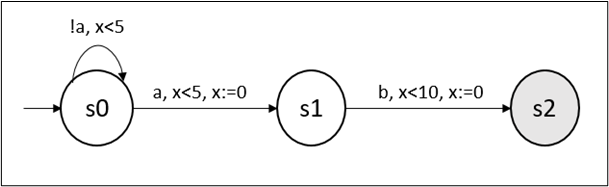
\includegraphics[width=130mm, keepaspectratio]{figures/9abra.png}
    \caption{Az összeállított automata.}
    \label{created_automaton}
\end{figure}

A monitor szempontjából az automata akkor jelez hibás működést ha olyan bemenetet kap, amely egyik élre sem illeszkedik.
Ilyenkor a követelmény már nem teljesíthető.
Ha az automata egy sima állapotban van, akkor az helyes működést jelent viszont a követelmény még ekkor sem teljesült.
A követelmény akkor teljesül amikor az automata a végső (\textit{FINAL}) állapotba kerül és nem érkezik további üzenet amely elmozditaná őt onnan.
A \ref{created_automaton} ábrán az „s2” szürke állapot a végsőállapot.